
\documentclass[preprint,12pt]{elsarticle}


%% The graphicx package provides the includegraphics command.
\usepackage{graphicx}
%% The amssymb package provides various useful mathematical symbols
\usepackage{amssymb}
\usepackage[utf8]{inputenc}
 % Added for the multi-column 
\usepackage[british]{babel}

% I added for arrows
\usepackage{textcomp}

\usepackage{hhline}
\usepackage{multirow}
\usepackage[figurename=Fig]{caption}
\usepackage{changepage}
\usepackage{listings}
\usepackage{color}
\usepackage{caption}
\usepackage{subcaption} 
\definecolor{codegreen}{rgb}{0,0.6,0}
\definecolor{codegray}{rgb}{0.5,0.5,0.5}
\definecolor{codepurple}{rgb}{0.58,0,0.82}
\definecolor{backcolour}{rgb}{0.95,0.95,0.92}
 
\lstdefinestyle{mystyle}{
    backgroundcolor=\color{backcolour},   
    commentstyle=\color{codegreen},
    keywordstyle=\color{magenta},
    numberstyle=\tiny\color{codegray},
    stringstyle=\color{codepurple},
    basicstyle=\footnotesize,
    breakatwhitespace=false,         
    breaklines=true,                 
    captionpos=b,                    
    keepspaces=true,                 
    numbers=left,                    
    numbersep=5pt,                  
    showspaces=false,                
    showstringspaces=false,
    showtabs=false,                  
    tabsize=2
}
 
\lstset{style=mystyle}
\usepackage{lineno}
% Added for the sub-pictures
\usepackage{subcaption}
\renewcommand{\thesubfigure}{\Alph{subfigure}}
% \biboptions{}

\journal{Journal Name}

\begin{document}
\vspace*{0.2in}

% Title must be 250 characters or less.
\begin{flushleft}
{\Large
\textbf\newline{Model checking vesicular transport system}}

Ankit Shukla, Kuppaswamy Lakshman 
\\
\bigskip
Chennai mathematical institute
\bigskip

% Use the asterisk to denote corresponding authorship and provide email address in note below.
* ankit@cmi.ac.in
* klachu@gmail.com
\end{flushleft}
% Please keep the abstract below 300 words

\section*{Abstract}
Modeling biological is an art. Biological systems are very complex in comparison to the computer system that we currently can build, for example a human body is a perfect example of the complexity involved in the system. So in order to understand these complex systems, besides experimenting the best way is to make simpler elegant model with suitable abstraction of biological systems and try to encode them as a computer programs. To understand the biological system we need some additional machinary besides simulation and stastical analysis. This paper presents two such model and proposed method that can handle the scalibilty problems and prdict precise results as opposed to a statistical one. We use model chekers (Boolean satisficability, SAT) as a framework to encode and analyze these model. We claim that these tools are suitable for biological systems which require combinotorial analysis of the stated rules and with possibly large state space.

\section{Fusion in eukaryotik cell}
The delivery of molecular cargo is essential for cell functioning and its survival. Specificity is required for essential functions in the cell for example sending signel to neighbouring nerve cell. Likewise, specificity is required for the export of hormones such as insulin to the cell surface. Intracellular organisation of eukaryotic cells is far more complex different from that of the prokaryotic cells. Distinct cellular processes in eukaryot are compartmentalised. This improves efficiency of the whole sytem but a critical problem surfaces. Now for the transport of the molecules different compartments need to exchange specific molecules and certain molecules need to be exported to the exterior of the cell. As its a case that most molecules are too large to directly pass through membranes, a mechanism is required to deliver the cargo from one compartement to another.

The process of vesicle transporting the cargo molecules can be thought as a several steps linear process (Fig.1) mainly involving:  
\begin{enumerate}
\item Sorting of cargo molecules from the source compartment for packaging into the vesicle.
\item Budding of the vesicle.
\item Uncoating and Tethering of the vesicle to the target compartment.
\item Vesicle fusion.
\end{enumerate}
We can understand the whole process of molecule transfer similar to that of a cargo transfer on a sea-shore. First step involves the sorting of the cargo molecules to be shipped, then cargo left for the target on a vesicle (small container of molecules) and at the end the cargo molecules shipped to its destination. With this basic picture few trivial question arises such as: how vesicle (cargo) finds (knows) its destination? Rothman, Schekman and Sudhof have discovered different parts of this mechninary, basically chemical specificity between SNARE's [0] dictates the fusion mechanism.

\begin{figure}[!ht]
  \caption{Mechanics of vesicle traffic sytem. The sequence of events that take place during vesicle-transport and the role of the major classes of traffic molecules is shown here.}
  \centering
   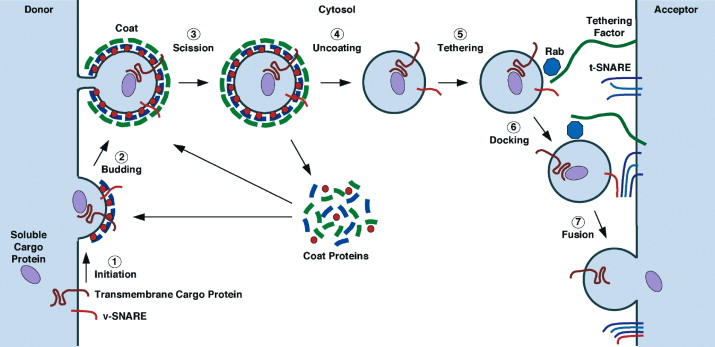
\includegraphics[width=0.95\textwidth]{2.jpg}
\end{figure}

Complete details of these process can be found at [1-6] and we'll assume that it's evident what is happening. 
 
\section{Introduction} Molecular interactions regulate the movement of transport vesicles between the membrane-bound compartments of eukaryotic cells [7]. Rothman, Schekman and Sudhof were awarded the Nobel Prize for identifying key molecules involved in this process. These include: Arf and Rab GTPases whose presence or absence encodes compartment identity [8]; coat proteins that regulate molecular loading from source compartments onto vesicles [7]; and SNARE proteins that regulate fusion of vesicles into target compartments [9].

These molecules form the basis of an abstract representation of vesicle traffic [10]: compartments are the nodes, and vesicles are the directed edges, of a transport graph; different molecules move in cyclical fluxes along this graph; the properties of compartments and vesicles are defined by the molecules they contain. 

In particular, we focus on the transmembrane SNARE proteins, which form a key part of the cellular addressing system. The fusion of a vesicle to a target compartment is driven by the zipping together of SNAREs [7;8]. In their fusion-competent state, SNAREs form a four-helix bundle: three components of this bundle are Q-SNAREs, the fourth is an R-SNARE. Both vesicles and their target compartments will contain SNAREs.

\section*{Cell evolution and color problem}
\subsection{Introduction }
\textit{Eukaryotic cells are filled with membrane-bound compartments, each of which has a characteristic size, shape and protein composition. During the life of the cell, proteins are constantly being transported inside vesicular carriers from one compartment to another, yet the structure and make-up of each compartment remain more or less constant. This implies that there must be a balance between outgoing and incoming
membrane traffic and, furthermore, that the cell must be able to transport proteins selectively, discriminating between proteins that need to move on to another compartment and proteins that need to remain behind. Thus, the process of vesicle formation must be tightly regulated, both quantitatively and qualitatively.}


\textit{Studies on clathrin-coated vesicles provided the first indication that the coat may serve two purposes: to deform the membrane into a budding vesicle and to select the contents of that vesicle.} Our focus will be on the second. 

We think the whole cell traffic network as a graph. In the topology of the graph, nodes are compartments of the molecules and molecules from one compartment to another travel via a smaller compartment (container) called vesicle. Vesicles carry molecules present on the source node and transfer them to the target compartment i.e only subset molecules present on the nodes are allowed to flow via vesicle. We can think this mechanism as molecule flow from compartments have some form of mask, i.e not all present molecules are allowed to go out on vesicle. We represent these vesicles as edges in the graph, the direction of the edge provides information about the source and target compartment and with every edge there is an associated mask. The whole vesicular system is a recyclable network. i.e every outgoing molecule is coming back to its original source node via a cycle. The problem is to come up with the minimized masks that is compatible with the valid system. 

\section{Color encoding problem}
Given a valid vesicle traffic system in which all molecules are recycled (i.e. all paths are cyclic) and all vesicles are distinct (3-connected \footnote{A graph is k-edge-connected if there does not exist a set of k-1 edges whose removal disconnects the graph (Skiena 1990, p. 177)}), what is the minimum number of coat proteins that are required. Abstractly, to find the minimum number of masks (we'll connect the coat proteins to mask of the traffic system in future sections) that is required in order to satisfy vesicle traffic rules in steady-state condition (molecules are recycled). 

\section{Previous work of use of formal methods in Biology}

Formal verification techniques are already used for aiding various
aspects of biological research [13-18]. In particular, the robustness of models of biochemical systems, modelling gene regulatory networks [18-20]. Our work is, to the best of our knowledge, the initial application of formal verification to studying the vesicle traffic regulatory networks also it opens up a novel application area for the formal verification community. With respect to related studies in simulation based vesile traffic system [10] our method can offer a higher degree of assurance, more accuracy, and better scalability than the traditional, simulation based approaches. 

Computing has contributed to the biological sciences by making it possible to store and analyze large amounts of experimental data. Recently, the development and application of computational methods and models that capture key biological processes and mechanisms is increasingly utilized towards helping biologists in gaining a clearer understanding of living systems and improving predictive capabilities. The ability to effectively explore and analyze such biological models is key to making scientific progress in the field.

\subsection{Overview of the model} There are two kinds of nodes in the system: compartments and vesicles. Compartments are all in steady state (recyclable). There are budding edges going from compartments to vesicles and fusion edges going from vesicles to compartments.

We describe coat proteins using two sets:
\begin{enumerate}
\item The set of molecules that the coat loads onto the vesicle (inclusion set, I)
\item The set of molecules that the coat avoids loading on the vesicle (exclusion set, E) 
\end{enumerate}

Whatever molecules from its inclusion set a coat finds on the source compartment, then it definitely loads it on the vesicle. If the source compartment contains molecules from the exclusion set of the
coat protein, then these molecules are not loaded onto the vesicle.
Since all molecules in the system are recycled, we identify molecules with the cycles on which they travel. In the model, we assign a single molecule to each elementary cycle of the traffic graph. Vesicle and compartment compositions are then given by the set of elementary cycles of which they are a part.
For each vesicle, we find the inclusion set (set of molecules that are present on the vesicle) and exclusion set (set of molecules present on the source compartment but not on the vesicle) for the
coat responsible.
We then define a coat incompatibility graph, where the nodes represent coats. Two nodes are adjacent if (I1 intersection E2) OR (I2 intersection E1) is not empty. The minimum number of colors in this graph represents the minimum number of coat proteins required in the system.

\textbf{Mathematical view} We can think this as a black box procedure. By solving the matrix multiplication procedure A mult B  where 2 - D matrix A represents the graph (1 in matrix : means  inflow -1 means outflow , others 0) and other 2-D matrix represent whether a type of molecule present at which compartment. Equating multiplication to a get stability condition cause whole cause representing them as equations form resulting into a form that implies that for stability there has to be cycles, vesicle flow over a cycle is conserved. 

\subsection{Modeling}
We modeled the system as a SAT problem by using \textit{bounded model checker CBMC (C-bounded model checker}. In comparison to simulation methods, model checking turn out to be very efficient way of solving this kind of problem. Rather than coding the properties directly we did some preprocessing to minimize the unwinding that CBMC takes. 

The input will be a graph where a node represents a compartment. Vesicle are moving out as edges. There is an inflow and outflow of the vesicles. With each possible edge, we assign a corresponding mask, that might not be unique. 

\textbf{Prob Statement:} In terms of graph representation problem can be viewed as: find the minimum number of mask that is required to make sure that following conditions are met:
\begin{enumerate}
\item System is in steady state (every graph cut balances inflow-outflow flux).
\item Underlying undirected graph is 3-connected.
\end{enumerate}

Steady state condition or homeostasis requirement for the whole system is the basis for recycling of SNARES. It states that every leaving molecule come back to its source node via a cycle. Mathematically it means that the network admits a non-negative cycle basis. 

\subsubsection{Mask}
Now consider associating with each possible edge a mask. That will determine the molecule outflow possibility.
 
Lets make a graph that have 3 Nodes representing three compartments . And 1 $\,\to\,$ 3 (inflow to Node three from 1) 3 $\,\to\,$ 1 {outflow from three to 1} 3 -$\,\to\,$ 2 {outflow from 3 to 2} , 1 $\,\to\,$ 2 , 2 $\,\to\,$ 1 hence total 5 Edges and three Nodes. 
Three Cycles are preset. 1 $\,\to\,$ 2 $\,\to\,$ 1, 1 $\,\to\,$ 3 $\,\to\,$ 1, 1 $\,\to\,$ 3 $\,\to\,$ 2 $\,\to\,$ 1. 

\begin{figure}[!ht]
  \caption{\textbf{Graph to describe the network structure.} The large circules in the graph represent compartments and the smaller ones are vesicles. we can see the all the possible cycles present in the graph. }
  \centering
   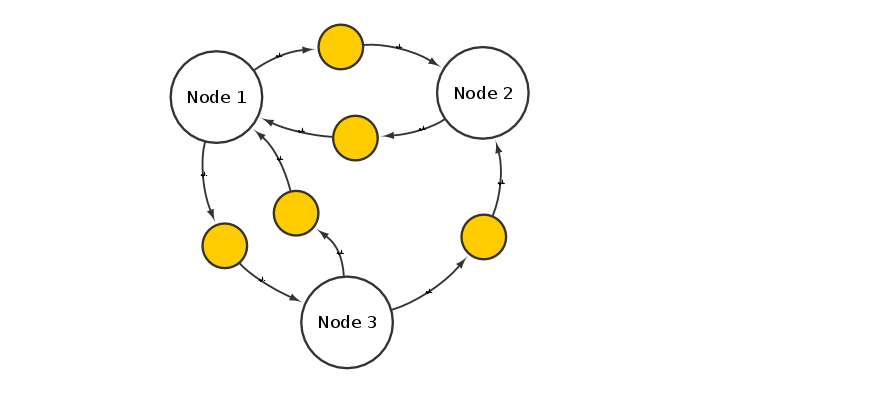
\includegraphics[width=0.90\textwidth]{1.png}
\end{figure}

There are substances that are present in at a compartment and few/all might be flowing through the a  edges and hence outgoing substance has to be present at the compartment. So we require in this case at least log 5 $\simeq$ 3 substances. 
Represent the matrix for the substance as a binary switch whether its present in a loop or not. 1 1 1 would mean that that substance is present at all the three loops. Reduce the binary switch to a graph coloring problem and solve the same to find the minimum required color. 

\subsection{Analysis}
Learning from our previous project where unwindings was really a problem and program was taking too much time before reaching into SAT solving phase we represented graph as 1 dimensional array which have edge between n and n+1\textsuperscript{th} element. 

\begin{figure}[ht]
%\vspace{-3mm}
\begin{verbatim}
# G[2N]: Graph with width twice as number of nodes.
# Graph is 3 connected.
#define N 5
#define X 2*N
...
unsigned int G[X];   
\end{verbatim}
\caption{Graph encoding.}
\label{code:motivate}
\end{figure}
 
 
 
This representation will cause additional book-keeping tasks but was very useful to decrease the loop unwinding in our code. In our Listing to illustrate the code with better readability we will assume that the graph is represented as a two dimensional matrix where G[i][j], G[i][j] = 1; there is an edge between node i and node j.

% \begin{lstlisting}[mathescape,
%   breaklines,
%   frame=single,
%   caption= \textbf{Readable encoding of the graph}
% ]
% #define N 5
% ...
% _Bool G[N][N];
% \end{lstlisting}

We represent nodes (compartments in the cell) in the graph as a bitvector of fixed length M (Total types of the molecules), representing information about the presence or absence of the molecule type at the i\textsuperscript{th} place.

We fix the graph as input. Then have created a preprocessing by making the edge as a C programming language structure, that consists of each node having additional information attached to it which we can later use by one lookup. The structure includes source and the target node i,j and bitvector representing the label of the edge (edgeWeight), chosen mask, inclusion and exclusion set. 
We can think edgeWeight as Boolean function with variable e\_{i,j,p} i,j range over to N (no of nodes) and p range from (0,5)


\begin{lstlisting}[language=Python,
mathescape,
 breaklines,
  rulecolor=\color{black},
  frame=single,
  caption= \textbf{Logical encoding of the edgeBag.}
]

edge = [[[ Bool ("e_{}_{}_{}".format(i,j,p)) for p in range(5)] for j in range(N)] for i in range(N)] 

\end{lstlisting}


\begin{figure}[ht]
%\vspace{-3mm}
\begin{verbatim}
# Define a structure to represent the EdgeBag that is a tuple :
# edgeBag := (i,j,edgeWeight,mask,inclusionSet,exclusionSet)

struct EdgeBag
 {
   int ith;
   int jth;
   bitvector edgeWeight;
   bitvector mask;
   bitvector inclusionSet;
   bitvector exclusionSet;
 };
 
....
# Create a structure that will contain edges. 
struct EdgeBag edgeBag[len];     

\end{verbatim}
\caption{Define a structure and represent edge with it.}
\label{code:motivate}
\end{figure}
 

But we still need and initiation of the structure. To initialize we just fix source and target node and allow rest to take an arbitrary value; i.e all possible assignments. Later we'll put constraint on these values and use variable involved in the property check.

\[ \bigwedge\limits_{i,j} g_{i,j} \supset (e_{i,j,0} == i \land e_{i,j,1} == j) \, \]

%\begin{lstlisting}[language=Python,
%mathescape,
% breaklines,
%  rulecolor=\color{black},
%  frame=single,
%  caption= \textbf{Steady state specification.}
%]
%\[ \bigwedge\limits_{i,j} g_{i,j} \supset (e_{i,j,0} == i \land e_{i,j,1} == j) \, \]
%
%\end{lstlisting}

\begin{figure}[ht]
%\vspace{-3mm}
\begin{verbatim}
# Set ith jth position and edgeweight to the position of
  edgeBag[len] array. 

edgePos = 0;
for(i = 0; i < N; i++) {
   for(j = 0; j < N; j++) {
        if (G[i][j] == 1) {
           edgeBag[edgePos].ith = i;
           edgeBag[edgePos].jth = j;
           edgePos = edgePos + 1;
        }
   }
}  
\end{verbatim}
\caption{Define the values of the source and target node according to the input graph.}
\label{code:motivate}
\end{figure}
 
The plan is simple; we constraint these variable values such that the system rules are followed. We do this by use of a Boolean variables and make that variable as a part of query to make sure that the assignment given after a run will be compatible with the rules specified. This way we can check properties about the system by making sure that basic rules are followed.  

\subsubsection{Steady state condition}
The steady state condition or homeostasis requirement for the whole system means that each molecule leaving the node on a vesicle should come back to its source node in a cycle, i.e., for every molecule leaving the node there exists a cycle with that molecule present on each of the edges and nodes of the path taken. 

We can state this specification regarding graph-cuts, that is each edge-graph-cut should maintain the inflow-outflow flux or as a property of assignment of molecules, such that each for each leaving molecule there is a cycle where that molecule is present on every edge and hops taken. Required Specification is listed in Listing 1. For efficiency reasons we'll divide the whole case into two as stated in last chapter.

\begin{lstlisting}[language=Python,
mathescape,
 breaklines,
  rulecolor=\color{black},
  frame=single,
  caption= \textbf{Steady state specification.}
]
# Every edge E is represented by a label; labelE (a bitvector).
# E(x,y): Edge between node x and y. E.source = x, E.target = y    
# labelE(m): mth molecule is present on edge E.
# Edge(m)(x,y): Edge between node x and y with labelE(m).                 
# seq(a1..an): each ak represents a node. len(seq) is |seq|.
# N: total number of nodes, = : Mathematical equality.
 
$\forall$ z $\in$ {Nodes} $\forall$ E $\in$ {Edges}: E.source = z $\supset$
    $\forall$ m $\in$ {Molecules}: labelE(m) $\supset$
       ($\exists$ a seq(a1..an): (2 $\leq$ |seq| $\leq$ N)  $\wedge$
            ((a1 = z) $\wedge$ (a2 = E.target) $\wedge$
             (($\forall$ k from 1 to |seq| - 1) $\supset$  Edge(m)(ak,ak+1)) $\wedge$
             (Edge(m)(an,a1)))

\end{lstlisting}

\subsubsection{Reduce the connection between the edges as 4 color problem based on inclusion and exclusion set}
Next we specify the inclusion and exclusion set for each edge that is present in the graph. W make sure that the edge  

\begin{figure}[ht]
%\vspace{-3mm}
\begin{verbatim}
# Specify inclusion and exclusion set for edge that is present in the graph.
# Add inside the condition of the mask structure possibility.
      
for(i=0; i < len; i++) {
      edgeBag[i].inclusionSet = edgeBag[i].edgeWeight;
      edgeBag[i].exclusionSet = nodes[edgeBag[i].ith] &
                                    (~ (edgeBag[i].ith)) ;
      
# Specify what are the possible configuration of the
# mask possible in the current setting.
# For any edge (mask & compartment config) == edge configuration. 
     __CPROVER_assume (( nodes[edgeBag[i].ith] & edgeBag[i].mask) 
                         == edgeBag[i].edgeWeight); 
}  
\end{verbatim}
\caption{Setting inclusion and exclusion masks.}
\label{code:motivate}
\end{figure}

\begin{figure}[ht]
%\vspace{-3mm}
\begin{verbatim}
# Making edge between the present edges to make it a coloring problem
for(k=0; k<len; k++) {
    for(l=0; (l<len); l++) {
         if(k == l) 
            colorGraph[k][l] = 0 ;
         else if ((( edgeBag[k].inclusionSet 
                     & edgeBag[l].exclusionSet) != 0) ||
                    ((edgeBag[k].exclusionSet
                     & edgeBag[l].inclusionSet) != 0) ) {
                    colorGraph[k][l] = 1;
		   }
		 else 
			 colorGraph[k][l] = 0; 
    }
} 
\end{verbatim}
\caption{Reducing the mask problem to n-color problem.}
\label{code:motivate}
\end{figure}


Solve four color problem to get the minimum color that is required to solve the prob.  

Have significance to Biology as cell contained max three or four color. 
     
     
Now we have to just solve the n color problem. There are many ways we can achieve simplest is shown in the Listing 

\begin{figure}[ht]
%\vspace{-3mm}
\begin{verbatim}
# Apply the constraints for the finding minimum coloring problem.
# Constraint1: all nodes are of some color.
# assignColor(C): C determined how many colors are given and 
  constraining C to be n we get whether its possible to restrict the 
  vesicle traffic system to be colored by n colors.
                   
for(i=0; i<len; i++){
     colorSet[i] = assignColor(C);
}

# Constraint2: If two edges are connected then both can't have same color.
C2 = 1;
for(i=0; i<len; i++){
	for(j=0;j<len;j++){
	     if(colorGraph[i][j] == 1) {
             C2 = C2 && (colorSet[i] != colorSet[j]); 
          }
    }
}
\end{verbatim}
\caption{Constraints for the n-color problem.}
\label{code:motivate}
\end{figure}


\subsection{Comparison with the simulation method}
Simulation method was able to handle the total number of nodes till N = 6. Scaling besides this limit was really a challenge. We checked every graph and achieved the same result and in some cases  

\section{Scalability and Discussion}
We have made our model abstract enough to work with model checkers and used the graph's structural properties to reduce the search space. We follow an approach that makes our code more scalable by restructuring the code that which suits some common knowledge about the code scalability.
\begin{enumerate}

\item[(i)] Decrease formula size and number of clauses: Generally, it is the thumb rule that if you have reduced formula size you have a better chance to find a counterexample. But this is not true all the time. We have used the technique to reduce the formula size by tweaking our code and in some places constraining system to search in a restricted search space. 

\item[(ii)] Avoid Variable coupling: Trying to minimize the number of connections or amount of interaction between variables helps a lot in a case where there are too many variables to solve for the SAT. Avoiding coupling is an important feature of the class of complex system we are trying to build, and it helped us in scaling this complex system up to 10 nodes.
\\ 
\end{enumerate}

\section{Conclusion}
\textbf{We find that the number of coats required in the system is much lesser than the number of vesicles made in that system.} The original goal was with the help of this model explain why only three or four coats colors are sufficient for the complex vesicle traffic system inside the eukaryotes. 

We were able to be solve biological problems far efficiently and with higher assurance (it can enumerate the all possible rules) and scalability specially in the color encoding problem where we able to do far better in comparison to the simulation methods. In both cases we were not able to predict and explain the complete behavior due to reasons specified earlier. One possible reason may be we still do not know enough about these system in terms of details of reasoning and also may have skipped/missed few important details while modeling the system itself. 

Most enthusiastic result of these project was some times model checkers performs far better in comparison to other times on some biological process and hence studying the important aspect that \textbf{why in certain case model checkers work might be connected to optimizations of the biology itself} is new path that future works can focus.  




\subsection{Introduction}
Central problem of cell biology is to understand the working of cell growth (and shrink). 

\section{Cell evolution basics}
SNARES are part of synaptic vesicle [Trimble, W. S. et al., 1988; Baumert, M. et al., 1989; Bennett et al., 1992] and their role in fusion mechanism is well established. They are proteins necessary for the fusion. We will focus on the mechanism of SNARE mediated fusion; a SNARE protein present on the vesicle membrane (v-SNARE) forms a complex with related SNAREs present on the target compartment (t-SNARE), resulting in docking the vesicle to the target compartment. One SNARE pairing in necessary and sufficient condition for the fusion [[Weber, T. et al., 1998]. 
SNARE traffic mechanism involves the following steps (Fig 1): 
\begin{itemize}
\item Pack V-SNAREs into outgoing vesicles at the source compartment.
\item Transport of these vesicles to their respective target compartments.
\item Fusion of vesicles with the target compartments by SNARE complex formation .
\end{itemize}

SNARE complexes are resolved into individual SNAREs by the action of the cytosolic proteins NSF and alpha-SNAP; these SNAREs can then be used for another round of fusion [Jahn, R., \& Scheller, R. H., 2006]. We know that the cell makes use of recycled SNAREs because blocking the reaction of NSF and alpha-SNAP eventually blocks secretion [Malhotra, V. et al., 1988]. But before the v-SNARE can be used in another round of fusion, it must first be sent back to its source compartment. Therefore, the picture we have so far of SNARE traffic is
incomplete in the sense that it does not include the mechanism of recycle of v-SNAREs. In this chapter, we present a possible mechanism of SNARE recycle that makes use of the molecular machinery discussed so far, and the repercussions of this mode of SNARE recycle on the global topology of the vesicle traffic network.

\begin{figure}[!ht]
  \caption{Figure 1: Schematic representation of the mechanism of action of SNAREs and SNARE-interactors. (A) Sequence of events that lead to the fusion of a vesicle with the correct target compartment: The source compartment produces a vesicle which contains v-SNARE molecules. This vesicle travels to the target compartment where the v-SNARE encounters its corresponding t-SNARE. The v-SNARE contributes a single SNARE motif and the t-SNARE contributes the rest of the three motifs required for the SNARE complex. The SM protein specific to these SNAREs oversees the assembly of the v- and t- SNAREs into a SNARE-complex. SNARE complex formation releases enough energy to enable vesicle fusion. (B) Post-fusion, the v- and t-SNAREs remain bound as a stable SNARE complex. Resolution of this complex into individual SNARE molecules requires the action of the ATPase NSF and alpha-SNAP.}
  \centering
%   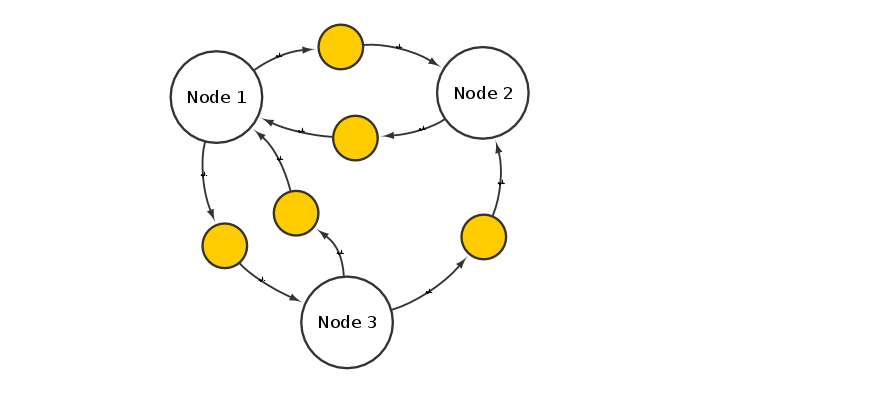
\includegraphics[width=0.65\textwidth]{1.jpg}
\end{figure}

% We model this process as a binary circuit and in process ask and learn additional properties of it as a Boolean satisfiability (SAT) problem. The classical way to attack this problem is to use simulations and analyze the results using statistical methods which are not very efficient and scalable and can not reason about all possible cases (as its hard to enumerate for all possible value/rules). We are going to use bounded model checkers (BMC) as a tool-framework to check and verify properties of interest. Model checker are most reliable in terms of precision but scalability of Model Checkers is always been an issue, here  we have shown it’s possible to scale the model checkers to model interestingly large complex biological systems as compared to simulations methods.

\section{Cell evolution as Boolean Circuit}
We are interested in modeling it as simple Boolean circuit [Mani-thattai] and understanding useful properties of the underlying system. Initial attempt has been made to model this Boolean circuit by using a simulation and taking average over the results. That experiment has been covered in Somya's [Mani] thesis completely. We have modeled the same system using the bounded model checker (BMC). We have used CBMC (C-bounded model checker) and abstracted away many details to make model as simple as possible and compute exhaustive solution. 

\subsection{Modeling as Boolean Circuit}
Cell can be thought as a container of compartments (eucaryotic cells) where each compartment contains molecules. We fix different types of molecule present in the system, upfront. So total possible different compartment are $2^{M}$. We are interested in how many different compartments are present and will not care about how many of similar compartments are there. So, a state will represent how many different compartments present in the cell. Doesn't care if two/more copies of the same compartment present. The system will start in an arbitrary state and using transition rules it will make a transition.

Considering a compartment as a subset of different types of molecules. The system is driven by two set of rules:
\begin{itemize}
\item Update Rules: Driven by an arbitrary M * M buddying matrix (absorption table).
\item Delete Rules: Driven by an arbitrary M * M fusion matrix (release table).
\end{itemize}
In terms of biology the budding matrix specifies which form of vesicles are allowed to go out from a compartment. One obvious restriction on vesicle that is allowed to go out is that it has to be a subset of the molecules present on the compartment. 


These tables will act as a rule for the update and deletion of the contents (molecules) from the compartments. There are total $2^{M * M}$ possible rules for given M * M matrix (table). In theory there is no restrictions on these tables beside a few obvious ones (eg. subset leaving requirement), but in practice we can assume that the budding matrix is constrained and at most two type of the vesicle is allowed to go out from a compartment. We impose no such restriction on the fusion matrix i.e for any vesicle coming to fuse the target compartment it is possible to so, if the matrix allows it. In both of these table, rows are compartments.

\textbf{State update (one iteration)}: Lets assume we have a current state specifying the total number of different compartment that the cell have. In the next step, set of compartments release vesicles (set of molecules) as dictated by release table. Every compartment can absorbs all those vesicles that it is permitted by the absorption table. Vesicles absorbed by one compartment must have been released in this iteration by some other compartment. These stages are concurrent: for each compartment C currently present, its behavior is determined by row C in both tables.
    
\textbf{ Creating new vesicles:} To create a new vesicle there is more than one possibility. Each released vesicle that is not used, becomes a new compartment. All vesicles that are released but not used merge to form a single new compartment.

Need not stick to the absorption/release table format for state update.  Can use any update rule that takes set of subsets of molecules to a new set of subsets.

Optimizations that make SAT solution go through may have interesting implications for biology, so useful to experiment with such optimizations regardless of their current biological significance.

\textbf{New interesting queries:} Count the number of equilibrium states for a given set of rules.

\subsection{Synchronous and asynchronous Model}
\subsubsection{Synchronous model}
Cell starts in the arbitrary initial state and the evolution is dictated by the two one step rules : update and delete. These update/delete can be performed in the on by one fashion who dictates the next state to achieve a specific state which of our interest. 

\subsubsection{Asynchronous model}
Rather than performing the task one step using either update or delete in one by one fashion we can allow the cell to be updated in asynchronous way and hence the next state is dictated by the way these two steps are performed.


Main Goal of David Dills Asynchronous Model was : To define timing robustness as the ability of cells to function correctly when there are significant variations in the timing of internal events, and explore timing robustness in cellular control systems using symbolic model checking.

\subsection{Implementation}
\subsubsection{Basic setup}
We model cell evolution as a transition function. Bounded model checker is very suitable for these type of encoding where we can check the property by fixing some lower bound and incrementing it thereafter to achieve the desired goal.

Lets fix different types of molecules present in the system (N). Hence the total number of possible different compartments can be $2^{N}$ lets call it M (power-set of N). 
As we consider only distinct compartments we can represent the state of the system as M bit length bitvector where each of the bits represent the different ith molecule and 0 or 1 represent their present or the absence.

\subsubsection{Example}
Lets Fix N = 2. Total number of molecules are two. Let's represent them as two different natural number 1,2. Total number of possible combination of N = $2 ^ {2}$  = 4 will be represented as 
\begin{itemize}
\item \{0\} : Represents Nothing is present. Compartment is empty.  
\item \{1\} : Represents A compartment with only one molecule 1 is present.
\item \{2\} : Represents A compartment with only one molecule 2 is present. 
\item \{1,2\} : Represents a compartment with both the molecules are present.
\end{itemize}

\subsubsection{Transition}
Starting from an arbitrary initial state and evolving (making progress from initial state) by using a transition function based on two tables
\begin{enumerate}
\item  Buddying Matrix : removes the materials from the cell compartments or completely delete a it (equivalent to a empty compartment).
\item Fusion matrix : adds some material (molecules) to the current compartment of the cell or adding new compartment.

\begin{itemize}
\item Prev State: \{\{1\}, \{2\}\} Next State:  \{\{1,2\}, \{2\}\}.
               Added molecule \{2\} to first compartment.    
\item Prev State : \{0\}: dead. Next state: \{1,2\} :
               Cell with a compartment having two molecules, 1 and 2.
\end{itemize}
\end{enumerate}
    
\subsubsection{Table representation}
 Both table have M * M dimension. M is total number of subsets for a given N.  For N = 2 i.e total $2^{2}$ = 4 subsets, hence M will be 4. We constraint the table to take only Boolean values and leave the value arbitrary, hence the possible values at any place of 2-dimensional table is either have 0 or 1. Value 0 represent no possibility to make a move. 1 represent move is allowed.  
 
Rules for Update and Deletion Tables del[M][M] , update[M][M]: 

\begin{enumerate}
\item For Update Table :
\begin{itemize}
\item Exactly One possibility in a single row to make progress.
        \item Basic Example : Update caused a compartment \{1\} to add molecule 2. Hence become compartment \{1,2\} in next state 
        \item Progress might be just staying there; i.e no molecule is added to the current compartment.
\item Like \{1\} $\mapsto$ \{1\} after an update state means compartment remained the same.
\end{itemize}

\item For Deletion Table :
\begin{itemize}
\item  At least one possibility in a single row for the deletion table.
\item Allow multiple possible deletes.
\item This might be used to model the situation based on non-deterministic choice.
\end{itemize}
      
\end{enumerate}
        
\begin{table}[]
\centering       
\label{my-label}
\begin{tabular}{l*{4}{c}r}
Compartment  & 00 & 01 & 10 & 11  \\
\hline
00 & 0 & 1 & 0 & 0     \\
01            & 0 & 0 & 0 & 1     \\
10           & 0 & 0 & 1 & 0     \\
11     & 0 & 0 & 0 & 1     \\ \\ 
\end{tabular}
\caption{Update table}
\end{table}

Lets see with the help of an example what are the possible cases. Lets analyse the results of a single update table rule. 

\begin{enumerate}
\item update[1][3] = 1 : means second row and forth column is = 1 and hence a valid move. As the rules are deterministic and there is only one choice if a compartment has this configuration \{1\} in next state molecule 2 will be added to this compartment and hence it'll become \{1,2\}. 
\item update[2][2] = 1 : means third row and third column has 1. Means in an update phase a molecule with configuration \{2\} will remains \{2\}. Nothing is going to be added. Stay on. 
\end{enumerate}

 Adding same molecule to the current compartment where already that molecule is present would have no change in configuration of the molecule. For example if we add molecule 1 to a compartment with configuration \{1,2\} its still be \{1,2\}. That means we are not taking care of count of same molecules present.\\\\
     
\begin{table}[]
\centering       
\label{my-label}
\begin{tabular}{l*{4}{c}r}
Compartment  & 00 & 01 & 10 & 11  \\
\hline
00 & 1 & 0 & 0 & 0     \\
01            & 1 & 1 & 0 & 0     \\
10           & 1 & 0 & 0 & 0     \\
11     & 1 & 0 & 1 & 0     \\ \\ 
\end{tabular}
\caption{Delete table}
\end{table}

For the delete table lets see what possibilities are there.
\begin{enumerate}
\item delete[0][0] = 1 : if molecule is dead nothing can be deleted from it.
\item delete[3][0] = 1 , delete[3][2] = 1 : means if compartment has this configuration \{1,2\} in deletion phase there will be a non-deterministic choice between these two options.
\begin{itemize}
\item delete[3][0] will give an effect (means) if compartment has configuration \{1,2\} before a delete phase in deletion phase this compartment will loose both elements and will become dead. i.e \{0\}
\item  delete[3][2] = 1 : It’ll give an effect (means) if compartment has configuration \{1,2\} before a delete phase in deletion phase this compartment will loose one element \{1\} and will become a compartment with only one molecule 2, \{2\}.
\end{itemize}
\end{enumerate}
 
Another assumption: In order to make the behavior consistent initially we enforce that only last choice will be taken i.e getting an effect that only last delete is present. Deletion will be carried out.eg: from \{1,2\} two possibilities:
\begin{itemize}
\item delete \{1\} and hence new compartment will have \{2\} remaining.
\item delete Both molecule and hence cell becomes dead to \{0\}.
\end{itemize}
 In this case b will be taken as the choice. 
 
\subsubsection{Encoding used:}

\textbf{Implementation of the functionality of the table:}
We have encoded the table functionality as a go-to table. Rather than using table to state which things can be deleted from the table we have encoded "what happen if something is deleted from the table". Meaning if" let's row 3 (representing \{1,2\}) and column 2 (representing \{2\}) have a value " 1 " i.e delete[i][j] == 1; from a compartment with \{1,2\} deleted {1} and we now left with a compartment with a only one element/material \{2\}. Which is kind of abstract meaning rather than a explicit form. This saves few additional computation that is required after we know which can be deleted. Intuitively we might have encode this as delete[3][2] == 1 means from \{1,2\} and \{2\} you delete \{2\} and somehow figure out (via some calculation  here trivial) to delete \{2\} from this compartment and transform this compartment to a single element compartment \{1\}.

 \textbf{States representation:}
States are represented using a Bitvector of length M. That means let's say N = 2 which have total possible $2^{2}$ = 4 those are \{0\}, \{1\}, \{2\}, \{1,2\}. state: 0100  (read from left side i.e from MSB) represent in  meaning only one compartment present i.e with element/material 1 (\{1)\}. 

Similarly 0111 means three compartment currently present  which are \{1\}, \{2\} and a \{1,2\} these are represented just by position (MSB rather than LSB yes it's unintuitive but will allow  us to use table representation as a bit vector as not possible in any form to tell computer what \{1,2\} really mean). First zero represent compartment with no element present \{0\} not mean much. First  1 represent a compartment with single element 1 (\{1\}). etc last one i.e LSB 1 rightmost one represent presence of a compartment with two elements \{1,2\}.
 
 The basic code is a loop which allows transitions to be made and then checks property of interest. Listing 1 shows the coded loop with the property that it will check for the lassos in the transitions system (using the variable state, next\_state,looped,on\_loop and with the help of transition() function able to make transition. \_\_CPROVER\_assert has been used to check the property of interest after one transition has taken place.   
 \begin{lstlisting}[language=Python,
mathescape,
 breaklines,
  rulecolor=\color{black},
  frame=single,
  caption= \textbf{Basic loop handling the transition with checking the property after one update.}
]
while(1){					   		 
    save = nondet_bool(); 			     
    if (save && (!saved)) {
        l2s_s = state ;           
    }	
     on_loop = (save || saved);			
     next_state = transition(state, getRel, getAbs);
     counter++;
     state = next_state;
     saved = on_loop;  
     looped = (saved && (state == l2s_s));
     if (on_loop && !looped) savecnt = counter;  
     __CPROVER_assert( (!(on_loop) ||  (!looped || savecnt >  10)), "every stable state is reached within 10 iterations");

}
\end{lstlisting}

 State will make transition based on the transition function which will take help from delete and update to make a transition  to next state. As it is possible to have a multiple one's in a row in deletion table we have to use some means to implement our most weighted delete a choice, here used that facility as getlastone() function. As the state representation is reverse i.e from MSB to LSB getlastone will mean implement most weighted delete. Which make the encoding consistent (we can think this as exactly one).

\subsubsection{Updated Model}
We employ few basic steps from our learning from the synchronous model. One it was too far from reality and we need to create abstraction to get away from all the required details and focus on large viewpoints. The basis of the project was to define an asynchronous model of the cell structure evolution by choosing right abstraction and verify properties to understand these system better, and if possible match against the experiment results in the labs. 

Underline:
\begin{enumerate}
\item We can abstract away from the concept of vesicle which is the  deviation from previous model where we were differentiating with the compartments and the vesicle.
\item Cell now have only compartments which grows and shrinks. 
\item Compartment can either fuse or breakup.
\item Only pairs fuse and breakup partitions the compartments in two different molecules.
\item Rather than just avoiding the identical compartments we enforce consideration of conservation of molecule.
\item We'll take count of no.of similar molecules present. Count will be relevant in case when there is total only one molecule (count = 1 for a molecule).
\item An asynchronous model of evolution will take place, asynchronous in terms that choice for which one you pick for an update or delete.
\item As we can implement it non-deterministically the probability of the choice between fuse and breakup are equal. So we bias the probability by a fixed rate to favor of fusion. eg : prefactor * No of distinct pairs allowed to fuse.
\item In case where total compartments are less than 4 we'll always do breakup and in case where total compartments are
   $\geq$ 100 we always do a fuse. So restricting the focus set. 
\item New compartments can be created via the breakup subset never get absorbed and leading to a creation of new compartment.
\item We have to find some evolution that is reproducible such that ordering of events does not matter. i.e the cell starting in certain configuration will end up in one configuration whichever way the ordering happened.
\end{enumerate}
% 1. No concept of vesicle now. Deviation from previous model where we were differentiating with the compartments and the vesicle.

% 2. Cell now have only compartments which grows and shrinks(Not sure about shrinking, I have not asked him 
%    to make it clear what happens when a compartment looses all elements, whether it dies(disappears) or wait 
%    for next step to gain few other elements , need to get flavour of {0} representation and neccesity of the same). I think he meant 
%    was compartment dies. 

% 3. Compartment can either fuse or breakup. 

% 4. Only pairs fuse and breakup partitions the compartments in two different molecules.  

% 5. Conservation of molecule is still undecided. (Yet To decide).

% 6. We'll take count of no.of similar molecules present. Count will be relavent in case when there is total
%    only one molecule (count = 1 for a molecule).
 
% 7. An asynchronous model of evolution will take place, asynchronous in terms that choice for which one you pick .

% 8. As we can implement it non-deterministically the probability of the choice between fuse and breakup are equal.
%    So we bias the probability by a fixed- Rate to favor one over the other (he said biased in favor of fuse).
%    eg : prefactor * No of distict pairs allowed to fuse etc.

% 9. In case where total compartments are less than 4 we'll always do breakup and in case where total compartments are
%    $\geq$ 100 we always do a fuse. So restricting the focus set. 
 
% 10. New compartments can be created via the breakup subset never get absorbed and leading to a creation of new compartment.
%    Or multiple unabsorbed get collected to create a new compartment. Not decided which one.

% 11. We have to find some evolution that is reproducible such that Ordering of events does not matter. 
%     i.e the cell starting in certain configuration will end up in one configuration whichever way the
%     ordering happened.

Two things still not clear in my mind.

In which sense he used the word molecules, it has a vesicle feeling? 
Multiple donor thing {I think he meant { more than a one donor creating a new compartment} } (forgot why that was so important). 

\subsection{Conclusion}
We have experimented with the synchronous update model and found that it was not very scalable.


\nolinenumbers

\end{document}

